\jxhj{%教学后记
	}
\skrq{%授课日期
	2018年1月11日 4-5节}
\ktmq{%课题名称
	 宏程序Z向分层}
\jxmb{%教学目标,每行前面要加 \item
	\item 掌握用循环来实现Z向分层;
	\item 掌握条件表达式的确定(加不加“=”);
	\item 掌握if then的使用;
	\item 掌握多个While的使用。
}
\jxzd{%教学重点,每行前面要加 \item
	\item if then的使用;
	\item 理解变量的分类。 }
\jxnd{%教学难点,每行前面要加 \item
	\item 条件表达式的确定。 }
\jjff{%教学方法
	通过讲述、举例、演示法来说明;}

\makeshouye %制作教案首页

%%%%教学内容
\subsection{组织教学}
\begin{enumerate}[\hspace{2em}1、]
	\item 集中学生注意力;
	\item 清查学生人数;
	\item 维持课堂纪律;
\end{enumerate}

\subsection{复习导入及主要内容}
\begin{enumerate}[1、]
\item 变量与常量;
\item Fanuc上的变量;
\item 变量的分类;
\item 算数运算;
\item 运算顺序与括号;
\item 加工实例。
\end{enumerate}

\subsection{教学内容及过程}
	
\subsubsection{Z向分层}
	基本思路:
	
	以前 G91+子程序
	
	G90 深度用 变量,每个深度进行计算。
	
	G91 次数用 变量,次数递增记数。
	
	形成循环。

\begin{lstlisting}
	#1=0
	N10 
	#1=#1+4
	G90 G1 z-#1
	……
	If [#1lt12] goto10
	
	#1=0
	N10
	#1=#1+1
	G91 g1 z-4.0
	……
	If [#1lt3] goto10
\end{lstlistting}	
	
	尽量用G90。
	
	思考一:

	如果初始值为4,侧程序怎么改

\begin{lstlisting}	
	#1=4
	N10 
	G90 G1 z-#1
	……
	#1=#1+4
	If [#1    12] goto10
\end{lstlisting}

	讨论分析:

	用  LE  

	结论: \#1=\#1+4 放在执行之前,判断的量是当前位置值,当前值为终点是,应结束循环,条件判断用 GT 或 LT

	\#4=\#4+4 放在执行之后,判断的量是下一个位置的值,下一点为终止值时,应走到终点后结束循环,条件判断应用GE或LE。

	思考二:当加工深度为13mm时怎么改程序。

	方法一:等分每层加工 13/4=3.25mm

	方法二:第一层加工1mm 其余12/4=3mm

	\#1=2    \#1=\#1-3

	注意初始值的更换。

	方法三:每层4mm 最后一层1mm

	怎么实现?

	\#1=0  \#1=\#1-4  到了16????

\subsubsection{IF  Then 指令}

	格式  if [条件] THEN [指令]

	功能: 条件成立时 执行 THEN 后的指令。

	条件不成立时,跳过后面的指令。

	如 if [\#1GT13] THEN \#1=13

	不适合判断的是下一个值,会干涉判断。

\subsubsection{Z向分层的应用}

\begin{lstlisting}
	#1=0
	N10 
	#1=#1+4
	If [#1 GT 13] then #1=13
	G90 G1 z-#1
	……
	If [#1lt13] goto10
\end{lstlisting}

	写成while就是:

\begin{lstlisting}
	#1=0
While [#1 lt 13] DO1
#1=#1+4
If [#1 GT 13] then #1=13
G90 G1 z-#1
……
END1
\end{lstlisting}


	实例:深度13
	
	如图\ref{fig:34-1}

\begin{figure}[h]
	\centering
	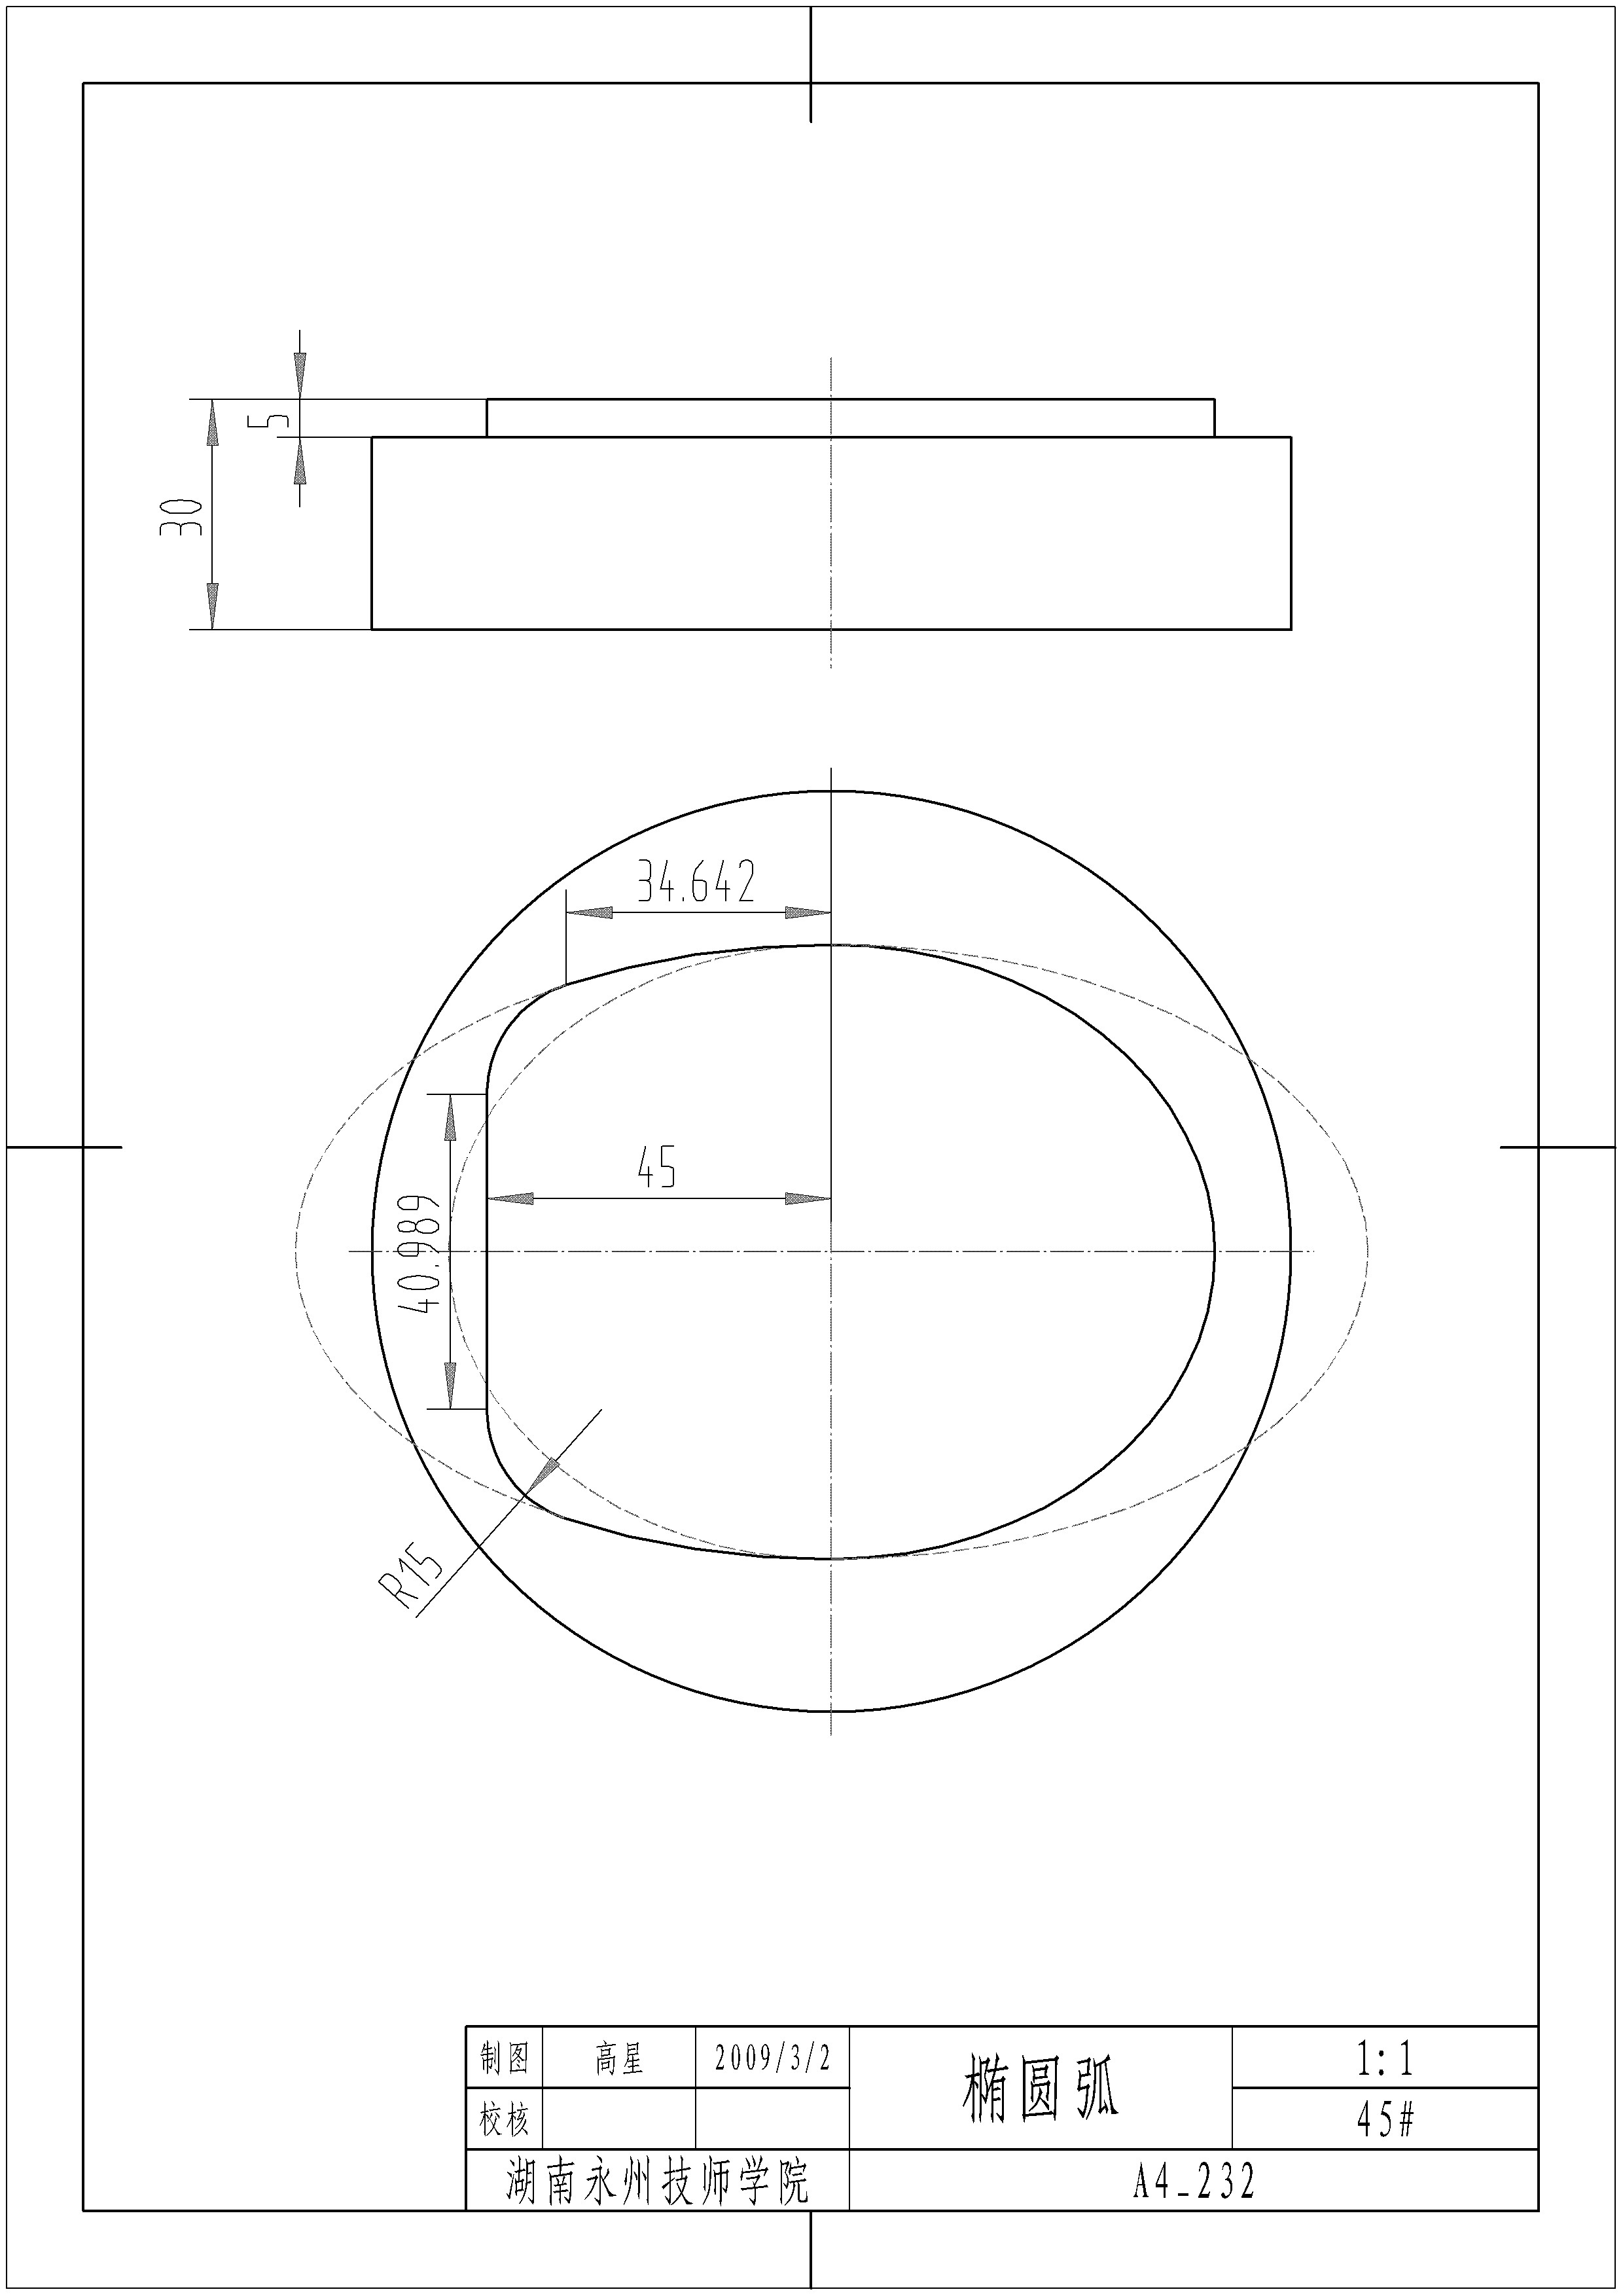
\includegraphics[width=0.7\linewidth,trim=50 150 50 100,clip]{data/image/34-1}
	\caption{加工实例}
	\label{fig:34-1}
\end{figure}
	

\subsubsection{多个While循环}  
	1、并列关系:
	
	While [条件] DO1
	
	……
	
	END1
	
	While [条件] DO1
	
	…… 
	
	END1
	
	也就是循环标识号可以相同。
	

	2、嵌套关系

	While [条件] DO1

	……

	While [条件] DO2

	…… 

	END2

	END1

	也就是循环标识号不能相同

	且最大嵌套3次,即 1、2、3。

\subsection{课堂小结}
\begin{enumerate}[1、]
\item Z向分层;
\item IF Then 指令;
\item Z向分层的应用;
\item 多个循环的应用。
\end{enumerate}

\vfill
\subsection{布置作业}
\begin{enumerate}[1、]
	\item 综合习题一。
\end{enumerate}
\vfill